\documentclass[xcolor=dvipsnames]{beamer}
%\documentclass{beamer}

%\documentclass[handout]{beamer}

%\usepackage[table]{xcolor}
\mode<presentation> {
  \usetheme{Boadilla}
%  \usetheme{Pittsburgh}
%\usefonttheme[2]{sans}
\renewcommand{\familydefault}{cmss}
%\usepackage{lmodern}
%\usepackage[T1]{fontenc}
%\usepackage{palatino}
%\usepackage{cmbright}
  \setbeamercovered{transparent}
\useinnertheme{rectangles}
}
\usepackage{soul}
\setbeamercolor{normal text}{fg=black}
\setbeamercolor{structure}{fg= black}
\beamertemplatesolidbackgroundcolor{white}  \setbeamercolor{alerted
text}{fg=red}
\usepackage{amsmath}
\usepackage[english]{babel}
\usepackage[latin1]{inputenc}
\usepackage{times}
\usepackage[T1]{fontenc}
\usepackage{colortbl}
\usepackage{framed}
\usepackage{color}
\definecolor{gold}{rgb}{0.85,0.66,0}
\usepackage{cancel}
\usepackage{comment}
\usepackage{enumerate}
\usepackage{multirow}
\usepackage{fancybox}

% === check mark
\usepackage{pifont}
\newcommand{\cmark}{\ding{51}}
\newcommand{\xmark}{\ding{55}}

% === tikz for pictures ===
\usepackage{tikz}
\usepackage[latin1]{inputenc}
\usetikzlibrary{shapes,arrows,trees,fit,positioning}

% ==== dotted lines in tables ===
\usepackage{arydshln}
\usepackage[normalem]{ulem}

% === dcolumn package ===
\usepackage{dcolumn}
\newcolumntype{.}{D{.}{.}{-1}}
\newcolumntype{d}[1]{D{.}{.}{#1}}

% === new commands ===
\newcommand\ud{\mathrm{d}}
\newcommand\dist{\buildrel\rm d\over\sim}
\newcommand\ind{\stackrel{\rm indep.}{\sim}}
\newcommand\iid{\stackrel{\rm i.i.d.}{\sim}}
\newcommand\logit{{\rm logit}}
\renewcommand\r{\right}
\renewcommand\l{\left}
\newcommand\Var{{\rm Var}}
\newcommand\var{{\rm var}}
\newcommand\Cov{{\rm Cov}}
\newcommand\bone{\mathbf{1}}
\newcommand\E{\mathbb{E}}
\newcommand\wX{\widetilde{X}}
\newcommand\wT{\widetilde{T}}
\newcommand\independent{\protect\mathpalette{\protect\independenT}{\perp}}
\def\independenT#1#2{\mathrel{\rlap{$#1#2$}\mkern2mu{#1#2}}}


 \newenvironment{changemargin}[3]{%
 \begin{list}{}{%
 \setlength{\topsep}{0pt}%
 \setlength{\leftmargin}{#1}%
 \setlength{\rightmargin}{#2}%
 \setlength{\topmargin}{#3}%
 \setlength{\listparindent}{\parindent}%
 \setlength{\itemindent}{\parindent}%
 \setlength{\parsep}{\parskip}%
 }%
 \item[]}{\end{list}}


\newcommand\bX{\mathbf{X}}
\newcommand\bB{\mathbf{B}}
\newcommand\bD{\mathbf{D}}
\newcommand\bM{\mathbf{M}}
\newcommand\bH{\mathbf{H}}
\newcommand\bI{\mathbf{I}}
\newcommand\bG{\mathbf{G}}
\newcommand\bR{\mathbf{R}}
\newcommand\bS{\mathbf{S}}
\newcommand\bV{\mathbf{V}}
\newcommand\bW{\mathbf{W}}
\newcommand{\argmin}{\operatornamewithlimits{argmin}}
\newcommand{\argmax}{\operatornamewithlimits{argmax}}
\newcommand{\indep}{\mbox{$\perp\!\!\!\perp$}}
\def\independenT#1#2{\mathrel{\rlap{$#1#2$}\mkern2mu{#1#2}}}
\DeclareMathOperator{\sgn}{sgn}
\newcommand\spacingset[1]{\renewcommand{\baselinestretch}%
{#1}\small\normalsize}
\newcommand\ex{\colorbox{princetonorange}{\color{princetonblack}\textsc{Example}} }
\definecolor{princetonorange}{RGB}{245, 128, 37}
\definecolor{princetonblack}{RGB}{0,0,0}

% == theorems
\setbeamertemplate{theorems}[numbered]
\newcounter{asm}
\setcounter{asm}{0}
\newtheorem{assumption}[asm]{Assumption}
\newtheorem{prop}{Proposition}

% === if you want more than one slides on one page ===
\usepackage{pgfpages}
%\setbeameroption{show notes on second screen}
%\pgfpagesuselayout{2 on 1}[letterpaper,border shrink = 5mm]

%%%%%%%%%%%%%%%%%%%%%%%%%%%%%%%%%%%%%%%%%%%%%%%%%%%%%%%%%%%%%%%%%%%%%%

% If you wish to uncover everything in a step-wise fashion, uncomment
% the following command:
%\beamerdefaultoverlayspecification{<+->}

\title[Machine Learning]{Machine Learning}
\author[Justin Grimmer]{Justin Grimmer}
\institute[University of Chicago]{University of Chicago}
\date{March 5th, 2018}

\begin{document}

\frame{\titlepage}


\begin{frame}
\frametitle{Causal Inference and Text}

\huge

\begin{itemize}
\item[-] Text as Treatment
\item[-] Text as Outcome
\item[-] Text as Confounder
\end{itemize}	


\end{frame}




\section{Text as Outcome}

\begin{frame}
\frametitle{Text as Outcome}
\begin{center}
\visible<2->{\includegraphics[height=.3\textheight]{twitter.jpg}}
\visible<3->{\includegraphics[height=.3\textheight]{survey2.jpg}}
\visible<4->{\includegraphics[height=.3\textheight]{twoheadlines.jpg}}
\end{center}

\begin{itemize}
\item<1-> Text is a rich source of information about the opinions, views and responses of individuals.
\item<5-> Most instances so far in political science of people collecting large text datasets have been text as \alert{outcome}
\item<6-> Also includes a long history of manual coding of open-ended survey responses and manual content analysis of documents.
\item<7-> We will define our estimand as:
\begin{align*}
E[g(Y_i(1)) - g(Y_i(0))]
\end{align*}
\end{itemize}
\end{frame}

\begin{frame}
\frametitle{Designing a $g$ Function}

\begin{itemize}
\item Before we can talk about learning the $g$ function, need to talk about desirable properties. \pause
\item Desirable properties of $g$ function \pause
\begin{enumerate}
\item \alert{Interpretable} \\
can we clearly communicate the idea to the reader \pause
\item \alert{Theoretical Interest} \\
helps us advance a relevant argument \pause
\item \alert{Label Fidelity} \\
minimal surprise when going from reading the label to reading the documents \pause
\item \alert{Tractable} \\
computationally tractable model and enough samples to estimate \pause
\end{enumerate}
\item We will consider unsupervised learning of $g$ function (works because unsupervised learning does dimensionality reduction)
\end{itemize}
\end{frame}

\begin{frame}
\frametitle{Types of $g$ Functions}

The biggest modeling choice is the form of the latent representation. \pause \\  There are many options: \pause

\begin{columns}[c]
\begin{column}{.3\textwidth}
\includegraphics<3>[width=.95\textwidth, page=1]{LatentRepTypes.pdf}
\includegraphics<4,7>[width=.95\textwidth, page=2]{LatentRepTypes.pdf}
\includegraphics<5>[width=.95\textwidth, page=3]{LatentRepTypes.pdf}
\includegraphics<6>[width=.95\textwidth, page=4]{LatentRepTypes.pdf}
\end{column}
\begin{column}{.7\textwidth}
\begin{itemize}
\item \alert<3>{Categorical}: one of $K$ mutually exclusive and exhaustive categories \pause 
\item \alert<4,7>{Mixed Membership}: proportional member of $K$ topics \pause 
\item \alert<5>{Binary Features}: $K$ binary latent variables, each of which could be one or off \pause
\item \alert<6>{Scales}: $K$ continuous scales or positions \pause
\end{itemize}
\end{column}
\end{columns}
\bigskip

We are going to use the Structural Topic Model (Roberts, Stewart and Tingley) which provides a mixed membership representation, but the exact method isn't important.

\end{frame}

\begin{frame}
\frametitle{Threats to Inference}

\pause
\begin{itemize}
\item If we have a $g$ function \alert{before seeing any documents} we have no problems. \pause
\item If not, how we \alert{discover} the $g$ function is important. \pause
\item When we use the same documents to discover $g$ (by manual or automated means) and estimate the treatment effect, we induce a \alert{dependence} across \alert{all} observations. \pause
\item Now $g(Y_i(\mathbf{T}))$ depends on all elements of $\mathbf{T}$ because treatment assignment of all documents affected our development of $g$. \pause
\item We call this problem an \alert{Analyst Induced SUTVA Violation}.
\end{itemize}
\end{frame}

\begin{frame}
\frametitle{Avoiding Analyst Induced SUTVA Violations}

AISVs are pernicious because they are exacerbated by what would otherwise be best practice. \pause

\medskip

Consider hand-coding: when we iterate between writing the codebook, classifying statements and analyzing intercoder agreement, we induce \alert{dependence}. \pause

\medskip

\begin{columns}[c]
\begin{column}{.35\textwidth}
\begin{center}
\includegraphics[width=.95\textwidth]{heroic.jpg}
\end{center}
\end{column}
\begin{column}{.65\textwidth}
We can avoid the AISV with a \alert{heroic} assumption that the codebook ($g$ function) doesn't depend on the specific randomization, i.e. that $g$ is \alert{stable} across all randomizations.
\end{column}
\end{columns}
\pause

\medskip

While this avoids the AISV, it doesn't remove concerns about \alert{fishing}.
\end{frame}

\begin{frame}
\frametitle{A General Solution: Train-Test Splits}

\pause
\begin{itemize}
\item We can address this problem by explicitly allowing for \alert{discovery} in the research process. \pause
\item Randomly partition sample into two sets: \alert{training} and \alert{test} \pause
\item \alert{Training Set}: do whatever we want to find the best $g$ function (useful and provides peace of mind).   \pause
\item \alert{Test Set}: Estimate causal effects using the learned $g$. \pause
\item This addresses:
\begin{itemize}
\item \alert{AISV}: $g$ does not depend on randomization in test set. \pause
\item \alert{Overfitting}: any fishing in training set will not produce result in test set.  \pause
\end{itemize}
\end{itemize}

\medskip

{\small Not coincidentally there is new functionality in the \texttt{stm} package that allows you to apply the $g$ function to a test set}
\end{frame}

\begin{frame}
\frametitle{Tradeoffs With Train-Test Splits}
\pause
\begin{itemize}
\item Train-test split is not costless: biggest concern is \alert{power}. \pause
\item It can be challenging to set the train-test split ratio because \alert{we don't know the power we need for discovery} \pause
\item We might also want to know that our discovery is invariant to the train-test split- although we note that it isn't strictly necessary. \pause
\item Also relies on the premise of well-intentioned actors who aren't `peeking' at the test set (although with outsourced data collection, some ways around this) \pause
\end{itemize}

\begin{framed}
We lose some power, but gain a process that preserves \alert{identification} of the causal effect.
\end{framed}
\end{frame}

\begin{frame}
\frametitle{Immigration Application: Experiment 1}

\begin{overlayarea}{\textwidth}{\textheight}
\begin{itemize}
\item<2-> Example application on a survey experiment about attitudes toward immigration.
\item<3-> Uses data from a study by Cohen, Rust and Steen (2004),  telephone random-digit dial of 1300 respondents (conducted in 2000). Train: $50\%$, Test $50\%$.
\item<6-> Respondents given a prompt about an immigrant, asked if she should be imprisoned and \emph{if they say no} why.
\end{itemize}

\begin{center}
\includegraphics<2-3>[width=.6\textwidth]{immigration.jpg}
\only<4->{
\includegraphics<4-5>[width=.45\textwidth]{bushgore.jpg} \includegraphics<5>[width=.45\textwidth]{mi2.jpg}
}
\only<7>{
\begin{framed}
``A 28-year-old single man, a citizen of another country, was convicted
of illegally entering the United States. Prior to this offense, he had
served two previous prison sentences each more than a year. One
of these previous sentences was for a violent crime and he had been
deported back to his home country.''
\end{framed}
}
\only<8>{
\begin{framed}
``A 28-year-old single man, a citizen of another country, was convicted
of illegally entering the United States. Prior to this offense, he had
never been imprisoned before.''
\end{framed}
}
\end{center}
\end{overlayarea}
\end{frame}


\begin{frame}
\frametitle{Immigration Application: Experiment 2}

\begin{itemize}
\item[-] Update sample using contemporaneous participants
\item[-] Alter the prompt: ``Should this offender be sent to prison?" (responses: yes, no, don't know) $\leadsto$ ``Why or Why not? Please describe in at least two sentences what actions, if any, the US government should take with respect to this person and why"  
\end{itemize}	


\end{frame}

\begin{frame}
\frametitle{Immigration Application: Experiment 3}

\begin{itemize}
\item[-] Examining Experiment 2: we noticed our labels were poorly constructed
\item[-] Cannot revise labels!
\item[-] Rerun experiment, team label the output
\end{itemize}	


\end{frame}


\begin{frame}

\only<1>{
\begin{scriptsize}
\begin{tabular}{r p{.4\textwidth} p{.4\textwidth}}
  \hline
 & Label & Highest Probability Words \\ 
  \hline
Topic 1 & Limited punishment with help to stay in country, complaints about immigration system & legal, way, immigr, danger, peopl, allow, come, countri, can, enter \\ 
  Topic 2 & Deport & deport, think, prison, crime, alreadi, imprison, illeg, sinc, serv, time \\ 
  Topic 3 & Deport because of money & just, send, back, countri, jail, come, prison, let, harm, money \\ 
  Topic 4 & Depends on the circumstances & first, countri, time, came, jail, man, think, reason, govern, put \\ 
  Topic 5 & More information needed & state, unit, prison, crime, immigr, illeg, take, crimin, simpli, put \\ 
  Topic 6 & Crime, small amount of jail time, then deportation & enter, countri, illeg, person, jail, deport, time, proper, imprison, determin \\ 
  Topic 7 & Punish to full extent of the law & crime, violent, person, law, convict, commit, deport, illeg, punish, offend \\ 
  Topic 8 & Allow to stay, no prison, rehabilitate, probably another explanation & dont, crimin, think, tri, hes, offens, better, case, know, make \\ 
  Topic 9 & No prison, deportation & deport, prison, will, person, countri, man, illeg, serv, time, sentenc \\ 
  Topic 10 & Should be sent back & sent, back, countri, prison, home, think, pay, origin, illeg, time \\ 
  Topic 11 & Repeat offender, danger to society & believ, countri, violat, offend, person, law, deport, prison, citizen, individu \\ 
   \hline
\end{tabular}
\end{scriptsize}
}


\only<2>{
\begin{eqnarray}
\widehat{ATE} %& = & E[g_{\boldsymbol{J}}(\boldsymbol{Y}_{i} (1) ) | T_i= 1]  - E[g_{\boldsymbol{J}}(\boldsymbol{Y}_{i} (0) ) | T_i= 0] \nonumber \\
& = & \sum_{i \in \boldsymbol{I} } \frac{ I(T_{i} = 1) g_{\boldsymbol{K}}(\boldsymbol{Y}_{i} (1  )  )   }{\sum_{i \in \boldsymbol{I} } I(T_{i} = 1 ) }  -  \sum_{i \in \boldsymbol{I} } \frac{ I(T_{i} = 0) g_{\boldsymbol{K}}(\boldsymbol{Y}_{i} (0  )  )   }{\sum_{i \in \boldsymbol{I}} I(T_{i} = 0 ) } \nonumber
 \end{eqnarray}
}

\only<3>{
\scalebox{0.5}{\includegraphics{2017TestEffects_Take2.pdf}}

}

\end{frame}



\begin{frame}

\Huge

How do presidents ``going public" affect public opinion?
\end{frame}


\begin{frame}

\begin{center}
\only<1>{\scalebox{0.45}{\includegraphics{ApprovalPlot.pdf}}}
\only<2>{\scalebox{0.45}{\includegraphics{MIP_Problem.pdf}}}
\only<3>{\scalebox{0.45}{\includegraphics{Topics.pdf}}}
\only<4>{\Huge How do presidents ``going public" affect \sout{public opinion} the media agenda?}


\only<5>{\scalebox{0.6}{\includegraphics{GoingPublicOverall.pdf}}}
\end{center}
\end{frame}


\begin{frame}

\Large

\begin{itemize}
\item[1)] (Assume) random assignment of treatments (use an interrupted time series design) \pause 
\invisible<1>{\item[2)] Obtain text based response $\boldsymbol{Y}_{i}(T_{i})$}
\end{itemize} \pause 

\invisible<1-2>{Function $g$ now uncovers latent features of response: map from text to small number of categories} \pause 

\invisible<1-3>{\begin{eqnarray}
\text{ATE}_{k} & = & \text{E}[ g(\boldsymbol{Y}(1))_{k} -g(\boldsymbol{Y}(0))_{k}] \nonumber 
\end{eqnarray}}


\end{frame}

\begin{frame}
\alert{Discovering (Estimating) Dependent Variable}

\Large
\begin{itemize}
\item[-] Numerous options to discover: (hand coding, supervised models, unsupervised models, mixture) \pause 
\invisible<1>{\item[-] \alert{All} have same worries: (1) Analyst Induced SUTVA violation (2) Overfitting (potentially via Fishing)} \pause 
\end{itemize}

\invisible<1-2>{\alert{Train/Test Split}} 


\end{frame}


\begin{frame}

\Large
\begin{itemize}
\item[1)] (Assume) random assignment of treatments
\item[2)] Obtain text based response $\boldsymbol{Y}_{i}(T_{i})$ \pause 
\invisible<1>{\item[3)] Randomly split response and text into train/test split} \pause 
\invisible<1-2>{\item[4)] In training set: discover latent dependent variables } \pause 
\begin{itemize}
\invisible<1-3>{\item[a)] Apply Structural Topic Model (Roberts, Stewart, and Airoldi 2017) }\pause 
\invisible<1-4>{\item[b)] Make final model pick based on quantitative model fit and exploration}\pause 
\end{itemize}
\invisible<1-5>{\item[5)] In test set:}\pause 
\begin{itemize}
\invisible<1-6>{\item[a)] Infer dependent variables (using newly available updates to {\tt STM} software (Roberts, Stewart, and Tingley 2017))}\pause 
\invisible<1-7>{\item[b)] Estimate effect of treatments on topic prevalence across categories}
\end{itemize}
\end{itemize}

\end{frame}

\begin{frame}

\Large 
A President's effect on newspaper agenda \pause 
\begin{itemize}
\invisible<1>{\item[-] Response: newspaper articles mentioning {\tt president} in 10 highest circulation papers, two-week window around speech} \pause 
\invisible<1-2>{\item[-] Treatment: Number of days before/after speech article was published} \pause 
\invisible<1-3>{\item[-] 159,217 articles} \pause 
\invisible<1-4>{\item[-] Train: 10\%, Test 90\%} \pause 
\invisible<1-5>{\item[-] Effect estimate: interrupted time series design on topic prevalence (compare share immediately before to share day after)}
\end{itemize}

\end{frame}


\begin{frame}

\begin{center}
\only<2>{\scalebox{0.65}{\includegraphics{AppealEffect.pdf}}}
\only<1>{\scalebox{0.65}{\includegraphics{Announce.pdf}}} 
\end{center}

\end{frame}


\begin{frame}

\huge 
Text as Confounder

\end{frame}


\begin{frame}
\frametitle{Selection on Observables}

Assumption:
\begin{itemize}
\item[] \alert{Random Assignment}: $T_{i} \indep Y_{i}(0), Y_{i}(1) $
\item[] \alert{Selection on Observables}:$T_{i} \indep Y_{i}(0), Y_{i}(1) | \boldsymbol{X}$ 
\end{itemize}

Text may be a confounder:
\begin{itemize}
	\item[-] Women are cited less in IR $\leadsto$ write about different subjects?
	\item[-] Chinese censorship increases blogging rates $\leadsto$ systematic differences in what is censored?
	\item[-] Radical cleric dying increases popularity of writing $\leadsto$ clerics targeted based on what they write?
\end{itemize}


\begin{itemize}
	\item[] \alert{Selection on Observables}: $T_{i} \indep Y_{i}(0), Y_{i}(1) | g(\boldsymbol{X})$
\end{itemize}

\end{frame}

\begin{frame}
\frametitle{Nielsen, Roberts, and Stewart(2018)}
\begin{itemize}
	\item[-] Maliniak, Powers, and Walter (2013)$\leadsto$ gender citation bias in IR
	\item[-] Causal question: \emph{same} article with man's name, different citation patterns?
	\item[-] NRS: use DFR from JSTOR $\leadsto$ 3,201 IR articles, 333 by women solo(!!!!)
	\item[-] Match using STM: estimate topics, coarsen exact matching, and then trimmed sample. (Use other matching procedures as well)
\end{itemize}
\end{frame}


\begin{frame}

\only<1>{\scalebox{0.5}{\includegraphics{DMRProjectionTopicsRichIR.pdf}}}

\vspace{0.5in}

\only<2>{\alert{Bigger} effect: 16 fewer citations for female articles.  (Na\"ive difference is 7)}


\end{frame}




\begin{frame}
\frametitle{Constituent Badges}

\huge

\pause 
\begin{itemize}
\invisible<1>{\item[-] Visually indicates that commenter is a constituent} \pause 
\invisible<1-2>{\item[-] Inspired by Capitol Hill focus groups} \pause 
\invisible<1-3>{\item[-] Survey responses from staff: identify constituents, we'll be responsive} 
% \item[-] Research Questions:
% \begin{itemize}
% \item[-] {\Large Does indication that a commenter is a constituent make reps more likely to reply?}
% \item[-] {\Large Does indication that a commenter is a constituent make other commenters more likely to reply?}
% \item[-] {\Large Do badges alter content of comments? }
% \item[-] {\Large Do badges increase repeated comments and who comments on elected officials' posts?}
% \end{itemize}
\end{itemize}


\end{frame}



\begin{frame}

\begin{tikzpicture}
\node (bad1) at (-7, 7) [] {\scalebox{0.4}{\includegraphics{Badge1.png}}};\pause
\invisible<1>{\node (bad2) at (-4, 7) [] {\scalebox{0.4}{\includegraphics{Badge2.png}}};} \pause
\invisible<1-2>{\node (bad3) at (-1, 7) [] {\scalebox{0.4}{\includegraphics{Badge3.png}}};} \pause
\invisible<1-3>{\node (bad4) at (2, 7) [] {\scalebox{0.4}{\includegraphics{Badge4.png}}};}
\end{tikzpicture}



\end{frame}

% \begin{frame}
% \frametitle{Constituent Badge Experiment}
% \begin{itemize}
% \item[-] 99\% treatment/1\% control group of U.S. users
% \item[-] Treatment = the ability to use and see others' constituent badges.
% \item[-] Control group = cannot badge themselves, cannot see other people's badges
% \item[-] Outcome metric: proportion of T and C groups that received like, reaction, or comment back from rep., other citizens
% \item[-] Point of exposure/randomization: see another user's (visible or invisible) badged comment or badging opportunity in Town Hall
% \item[-] Analyze `full complier constituents':
% \begin{itemize}
% \item[-] Treatment: constituents who adopted badge and commented on reps' pages
% \item[-] Control: constituents who commented on reps' pages
% \end{itemize}
% \end{itemize}
% \end{frame}


\begin{frame}

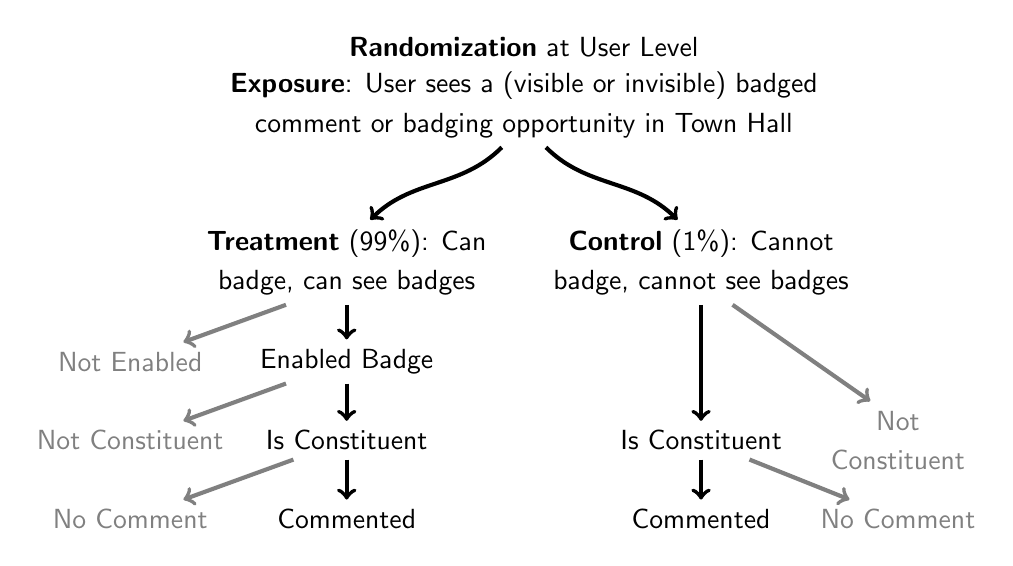
\begin{tikzpicture}
\node (dummy1) at (-7, 7) [] {} ;
\node (random) at (-1, 10.5) [] {\textbf{Randomization} at User Level}; 
\node (con1) at (-1, 10) [] {\textbf{Exposure}: User sees a (visible or invisible) badged } ;
\node (con2) at (-1, 9.5) [] {comment or badging opportunity in Town Hall} ;
\node (treat1) at (-3.25, 8) [] {\textbf{Treatment} (99\%): Can };
\node (treat1a) at (-3.25, 7.5) [] {badge, can see badges};

\node (control1) at (1.25, 8) [] {\textbf{Control} (1\%): Cannot };
\node (control1a) at (1.25, 7.5) [] {badge, cannot see badges};


\node (NE1) at (-6, 6.5) [] {{\color{gray} Not Enabled}} ;
\node (E1) at (-3.25, 6.5) [] {Enabled Badge} ;

\node (NE2) at (-6, 5.5) [] {{\color{gray} Not Constituent}} ;
\node (C1) at (-3.25, 5.5) [] {Is Constituent} ;

\node (C2) at (1.25, 5.5) {Is Constituent};
\node (NEC2) at (3.75, 5.75) {\color{gray}Not };
\node (NEC2a) at (3.75, 5.25) {\color{gray}Constituent};


\node (NE3) at (-6, 4.5) [] {{\color{gray} No Comment}};
\node (comm1) at (-3.25, 4.5) [] {Commented} ;

\node (NEC3) at (3.75, 4.5) [] {\color{gray} No Comment} ;
%\node (NEC3) at (4, 4.25) [] {\color{gray} Comment} ;
\node (comm2) at (1.25, 4.5) [] {Commented} ;


%\invisible<1-3>{\node (treat2) at (-4, 4) [] {Enabled Badge} ;}

\draw[->, line width = 1.5pt] (con2) to [out = 225, in = 45] (treat1);
\draw[->, line width = 1.5pt] (con2) to [out = 315, in = 135] (control1);
\draw[->, line width = 1.5pt, gray] (treat1a) to (NE1) ;
\draw[->, line width = 1.5pt] (treat1a) to (E1) ;

\draw[->, line width = 1.5pt, gray] (E1) to (NE2) ;
\draw[->, line width = 1.5pt] (E1) to (C1) ;

\draw[->, line width = 1.5pt] (control1a) to (C2);

\draw[->, line width = 1.5pt, gray] (control1a) to (NEC2) ;


\draw[->, line width = 1.5pt] (C1) to (comm1) ;
\draw[->, line width = 1.5pt, gray] (C1) to (NE3) ;

\draw[->, line width = 1.5pt] (C2) to (comm2) ;
\draw[->, line width = 1.5pt, gray] (C2) to (NEC3);

%\invisible<1-3>{\draw[->, line width = 1.5pt] (treat1) to (treat2);}
\end{tikzpicture}

\vspace{0.25in}

\Large \pause 
\invisible<1>{Focus on Intent to Treat Effects }

\end{frame}



\begin{frame}
\frametitle{Who Enables the Badge?}
Among Users who Interact with Politicians
\only<1>{\Large
\begin{tabular}{l|ccc}
         & \% Female &  Age & Facebook Friends \\
         \hline
  Badged & 54.3 & 53.9 & 395.0  \\
  Not Badged  & 46.5 & 49.1  & 475.5 \\
  \hline
  \end{tabular}
}

Aligns with survey-based evidence in Bode (2016)

\end{frame}



\begin{frame}
\frametitle{Badging Does Not Increase Politician Replies}

% \begin{tikzpicture}
% \node (dummy) at (-7, 7) [] {} ;
% \node (graph1) at (-2, 7) [] {\resizebox{3in}{2.5in}{\includegraphics{Effect1.png}}};
% \node (pie1) at (-7.5, 4.5) [] {\scalebox{0.4}{\includegraphics{Pie1.png}}};
% \node (text1) at (-8.5, 10) [] {Treatment: 3.10\% }  ;
% \node (text1a) at (-8.5, 9.5) [] {95\% CI [3.05, 3.15]};
% \node (text2) at (-8.5, 9) [] {Control: 3.07\% };
% \node (text2a) at (-8.5, 8.5)  [] {95\% CI [2.57, 3.58] } ;
% \end{tikzpicture}
%
\begin{center}
\scalebox{0.5}{\includegraphics{AdminEngagement2.png}}
\end{center}


\end{frame}



\begin{frame}
\frametitle{No Heterogeneity By Office}

ITT Effects By Office
\begin{center}
\begin{tabular}{l|cc}
\hline \hline
Office & Like & Comment \\
\hline
Overall & 0.0002 & -0.0003 \\
        &   [-0.0002, 0.0005]    & [-0.0007, 0.0000]\\
\hline\hline
Mayor & 0.003 & -0.000 \\
      & [0.0031,0.0035] & [-0.000, 0.000] \\
\hline
State & -0.0001            & -0.0003 \\
Lower &  [-0.001, 0.0008]  & [-0.001, 0.0005] \\
\hline
State    & \textbf{0.0052} & \textbf{-0.006} \\
Upper   & [0.004, 0.006]&  [-0.007, -0.005] \\
\hline
Governor & \textbf{-0.0008} & \textbf{-0.0002} \\
        & [-0.0003,-0.0001] & [-0.0009, -0.0006] \\
        \hline
House   & 0.0001 & -0.0014 \\
        & [-0.0016, 0.0013] & [-0.0001, 0.0003] \\
        \hline
Senate  & 0.0001 & 0.0000 \\
        & [0.0001,0.0001] & [0.0000, 0.0000] \\
        \hline\hline
\end{tabular}
\end{center}

\end{frame}

\begin{frame}
\Large

Why? \pause 
\begin{itemize}
  \invisible<1>{\item[-] Bad product, elected officials confused} \pause 
  \invisible<1-2>{\item[-] Constituents are not actually important } \pause 
  \invisible<1-3>{\item[-] Information matters, not on site}
\end{itemize}



\end{frame}



\begin{frame}
\frametitle{Elected Officials Write Longer Posts When They Do Respond}

\begin{itemize}
\item[-] Depart from Experimental Design
\item[-] Elected officials write longer posts $\leadsto$ more effort
\item[-] Examine how much longer responses are to \alert{badged} comments
\end{itemize}

\end{frame}


\begin{frame}
\pause 

\invisible<1>{\begin{center}
\begin{tabular}{l|ccc|ccc}
\hline \hline
Variables         & \multicolumn{3}{c}{Count} & \multicolumn{3}{c}{Log(Count + 1)} \\
\hline
Badged            & 5.96   & 4.4     &  2.2    &  0.24  &  0.20    & 0.08 \\
                  & (0.57) & (0.64)  &  (0.67) &  (0.02)&  (0.02)  & (0.02)  \\
Comment Length    &  -     & 0.2      &  0.14  & -      &  0.01    & 0.01   \\
                  &  -     & (0.01)   & (0.01) & -      &  (0.00)  & (0.00)  \\
USA Location    &  -     & -0.03    & 1.84   & -    &   -0.03  & 0.08    \\
          &  -     &  (0.48)  &  (3.3) & -    &   (0.01) &  (0.09)   \\         
\hline
Text Topics       &  No    & Yes      & Yes    &  No  & Yes   & Yes     \\
Positive      & No     & Yes      & Yes    &  No  & Yes   & Yes    \\
Negative      &  No    & Yes      & Yes    &  No  & Yes   & Yes    \\
Political Words    &  No.  & Yes      & Yes    &  No  &  Yes      & Yes  \\
Politician Fixed  &  No    &  No      & Yes    &  No    & No        & Yes \\
Effects           &        &          &        &        &       & \\
\hline \hline
\end{tabular}
\end{center}}


\end{frame}



\begin{frame}
\frametitle{Wrap Up}

\begin{itemize}
\item[-] Text as Data: Discovery, Measurement, and Causal Inference
\item[-] \alert{Lots} or ongoing research in this area!
\item[-] Applications to many non-text settings
\item[-] Intersects with many other areas
\end{itemize}	





\end{frame}








\end{document}



